\input{../../../permve-ntnu-latex/assignment.tex}

\usepackage{float}

\title{	
\normalfont \normalsize 
\textsc{Norwegian University of Science and Technology\\IT3105 -- Artificial Intelligence Programming}
\horrule{0.5pt} \\[0.4cm]
\huge Module 4:\\ Using Minimax with\\ Alpha-Beta Pruning to play 2048\\
\horrule{2pt} \\[0.5cm]
}

\author{Per Magnus Veierland\\permve@stud.ntnu.no}

\date{\normalsize\today}

\begin{document}

\maketitle

\section*{Branching factor}

The aim of module~4 is to achieve a winning score in the game \textsc{2048}. The game consists of a two-dimensional $4\times 4$ grid where each tile in the grid is either empty or has a number between $2^1$ and $2^{17}$ (inclusive). An upper bound of the game's branching factor can be found by multiplying the number of possible player moves~(4) by the maximum number of empty tiles~(16) by the number of possible tile spawns~(2):

\begin{displaymath}
b_{\textit{upper}} = 4 \cdot 16 \cdot 2 = 128
\end{displaymath}

\section*{State representation}

Given such a large branching factor for each player move it is evident that a large number of states must be evaluated to perform even a shallow search involving a low number of moves. To enable a large number of states to be considered an efficient state representation scheme is beneficial.

Even if the theoretical maximum tile is $2^{17}$, the largest tile required to win the game, 2048, is only $2^{11}$. Given that the number 1 is not present in the game, it is possible to represent the empty tile and tiles for powers of two between $2^1$ and $2^{15}$ by using 4~bits to represent each tile. With 4~bits reserved for each tile, all 16~tiles can be represented by a single 64-bit integer. Using a commonly available 64-bit processor architecture, each board state can be held in a single CPU register.

The resulting representation is shown in Figure~\ref{figure:represent} showing tile values and the corresponding bit values.

\begin{figure}[H]
\centering
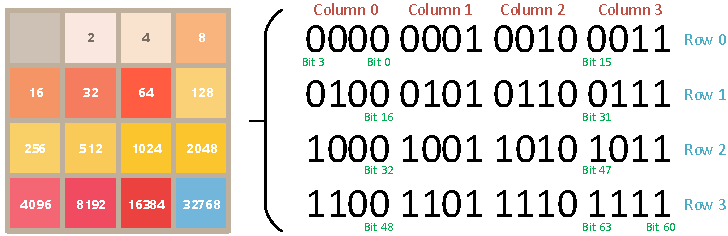
\includegraphics[scale=1.0]{images/2048_state}
\caption{64-bit integer state representation}
\label{figure:represent}
\end{figure}

\section*{Lookup tables}

Another benefit from the compact state representation is that it allows for efficient use of lookup tables. The logic necessary to compute the successor state when given a move requires loops and branches. The effect of performing a move is also local to each row or column, depending on the direction of the move. Each row or column can then be considered in isolation and depend on the exact same logic to produce their successor. The number of possible rows or columns is $2^{16}=65536$, so representing a lookup table for a single direction will take $2^{16}*8=524288$~bytes, or $0.52$~MB. By using four lookup tables, one for each direction, successor states can be evaluated by performing four lookups, one for each row or column.

Lookup tables can also be used to evaluate both board heuristics and board scores. The board heuristic may be a costly function to evaluate, making it very beneficial to pre-compute. However, unlike the state transitions which can be considered as functions considering each row and column individually, the heuristic function evaluates the entire board state. Since a lookup table containing entries for all states would be $2^{64}*8=18.45$~exabytes, this is currently infeasible. However by imposing the limitation that the heuristic function can only consider a single row or column at a time, only a single lookup table with $2^{16}$ entries is needed. This limits the information available to the heuristic function, but the implemented heuristic function is still able to provide sufficient guidance to the search. When evaluating the heuristic value for a state; 8~lookups are performed, one for each row and column, and the result is summed. The advantage of this approach is that the heuristic evaluation can use very costly operations in the pre-computation, since the evaluation only consists of lookups.

\section*{Expectimax}

The algorithm used to solve \textsc{2048} is \textit{Expectimax} with pruning based on a probability threshold and a transposition table. The code centers around the two functions \texttt

\section*{Software structure}

\section*{Heuristic}

Talk about split heuristic and disadvantages.

\end{document}

